\section{Preuve degré 5}

\begin{theorem}
  Soit un sggi de rang sur $A_{11}$. Alors ce sggi contient exactement une 4-transposition.
\end{theorem}

\begin{theorem}
  Soit un sggi sur $A_11$ de rang 5. L'unique 4-transposition de ce sggi est $\rho_2$.
\end{theorem}

\begin{proof}
  Il n'est pas possible que la transposition se trouve en $\rho_0$. En effet cela signifierait que $\rho_0$ doit commuter avec $\rho_2$, $\rho_3$ et $\rho_4$. Mais ceci est impossible car on a pas assez d'arêtes (voir la preuve du théorème suivant).

  \paragraph{}
  Si l'involution sur situe en $\rho_1$, alors elle doit commuter avec $\rho_3$ et $\rho_4$. Une d'elle doit former un carré alterné l'autre doit doubler une arête et relier deux points encore fixes. Pour $\rho_4$, s'il forme un carré avec $\rho_1$, on ne pourra le relier avec rien car il y deux involutions entre $\rho_1$ et $\rho_4$ et non une. Si par contre $\rho_4$ double un arête et relie deux points fixes. Alors ces deux points nouvellement reliés ne pourront jamais être reliés au reste du graphe car l'involution $\rho_3$ forme un carré alterné et n'est donc pas disponible.
\end{proof}

\begin{theorem}
  Soit un sggi de rang 5 sur $A_{11}$. Alors ce sggi n'est pas un C-group.
\end{theorem}

\begin{proof}
  Partons d'un diagramme avec juste la 4-transposition.

  \begin{figure}[H]
    \begin{center}
      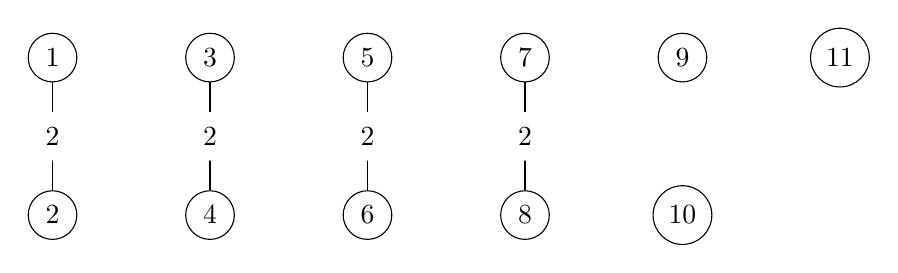
\begin{tikzpicture}

        \begin{scope}[every node/.style={circle,draw}]
          \node (1)  at (0,2)  {1};
          \node (2)  at (0,0)  {2};
          \node (3)  at (2,2)  {3};
          \node (4)  at (2,0)  {4};
          \node (5)  at (4,2)  {5};
          \node (6)  at (4,0)  {6};
          \node (7)  at (6,2)  {7};
          \node (8)  at (6,0)  {8};
          \node (9)  at (8,2)  {9};
          \node (10) at (8,0)  {10};
          \node (11) at (10,2) {11};
        \end{scope}

        \begin{scope}[every node/.style={fill=white,circle}]

          \begin{scope}[every edge/.style={draw}]
            \path (1)  edge node {$2$} (2);
            \path (3)  edge node {$2$} (4);
            \path (5)  edge node {$2$} (6);
            \path (7)  edge node {$2$} (8);
          \end{scope}
        \end{scope}

      \end{tikzpicture}
      \caption{[1, 5, 1010, 232, 381]}
    \end{center}
  \end{figure}

\paragraph{}
Nous allons essayer d'ajouter les involutions $\rho_0$ et $\rho_4$. Celles-ci doivent commuter avec $\rho_2$. Pour chaque involution nous devons choisir entre les 3 possibilités suivantes:
\begin{enumerate}
  \item Faire un arête double avec $\rho_2$ et reliés deux points qui sont, pour le moment, fixes.
  \item Faire deux arêtes doubles avec $\rho_2$.
  \item Faire un carré alterné avec $\rho_2$.
\end{enumerate}

\paragraph{}
S'il n'y a qu'une seule 4-transposition, alors nous avons 12 arêtes pour relier 11 points soit 2 de plus que le strict minimum. Sauf pour deux arêtes nous devons toujours relier deux composantes connexes différentes. Quand nous faisons un carré, nous utilisons une de ces deux arêtes et il se passe la même chose quand nous utilisons une arête double.

\paragraph{}
Nous ne pouvons jamais faire le second choix pour une involution car sinon nous aurions déjà utilisé nos deux arêtes et nous ne pourrions plus nous occuper de la seconde.

\paragraph{}
Remarquons qu'il est impossible de faire le même choix pour $\rho_0$ et $\rho_4$. Dans le premier cas, on aurait pas assez de point fixes. Dans le troisième cas, nous ne pouvons pas utiliser le même carré car cela formerait des arêtes doubles et donc il faudrait 3 arêtes libres. Il est impossible de faire deux carrés adjacents

\paragraph{}
Nous ne pouvons utiliser deux carrés adjacents car nous aurions une involution $\rho_0$ et $\rho_4$ adjacente mais nous avons déjà utilisé toutes les arêtes de ces involutions donc nous pouvons pas avoir un sggi.

\paragraph{}
Dans le cas deux deux carrés disjoints, nous ne pouvons pas les relier car il ne nous reste que des involutions $\rho_1$ et $\rho_3$ et celles-ce ne peuvent être adjacentes sans former un carré mais ça c'est impossible.

\paragraph{}
La seule possibilité qu'il nous reste est de choisir que $\rho_0$ reliera deux point fixes et doublera une arête et que $\rho_4$ formera un carré alterné. On a donc le graphe suivant.


\begin{figure}[H]
  \begin{center}
    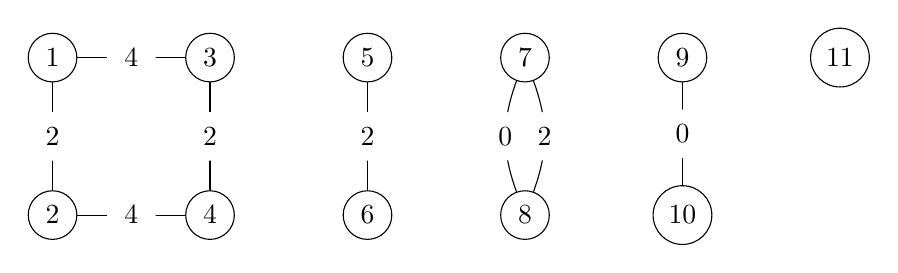
\begin{tikzpicture}

      \begin{scope}[every node/.style={circle,draw}]
        \node (1)  at (0,2)  {1};
        \node (2)  at (0,0)  {2};
        \node (3)  at (2,2)  {3};
        \node (4)  at (2,0)  {4};
        \node (5)  at (4,2)  {5};
        \node (6)  at (4,0)  {6};
        \node (7)  at (6,2)  {7};
        \node (8)  at (6,0)  {8};
        \node (9)  at (8,2)  {9};
        \node (10) at (8,0)  {10};
        \node (11) at (10,2) {11};
      \end{scope}

      \begin{scope}[every node/.style={fill=white,circle}]

        \begin{scope}[every edge/.style={draw}]
          \path (9)  edge node {$0$} (10);
          \path (7)  edge[bend right=20] node {$0$} (8);
          \path (1)  edge node {$2$} (2);
          \path (3)  edge node {$2$} (4);
          \path (5)  edge node {$2$} (6);
          \path (7)  edge[bend left=20] node {$2$} (8);
          \path (1)  edge node {$4$} (3);
          \path (2)  edge node {$4$} (4);
        \end{scope}
      \end{scope}

    \end{tikzpicture}
    \caption{[1, 5, 1010, 232, 381]}
  \end{center}
\end{figure}

\paragraph{}
À partir de maintenant, si nous rajoutons une arête, elle doit relier deux composantes connexes distinctes du graphe.

\paragraph{}
Vu l'impossibilité de former de carré, si nous voulons relier les involutions contenant $\rho_0$, nous devons utiliser $\rho_1$. Ces involutions devront être reliées à des involutions $\rho_2$ sinon ne ne pouvons plus étendre cette composante. Mais il n'est pas possible de relier au carré alterné car alors on aurait une paire d'involution $\rho_1, \rho_4$ adjacentes. Il y a donc une arête $\rho_1$ pour relier les deux composantes contenant $\rho_0$ et une autre pour relier ce tout à la composante $\{5,6\}$.

\paragraph{}
Il y a deux possibilités pour le sens dans lequel nous attachons à la composante $\{5,6\}$. Soit nous attachons par le côté où il y a l'arête double ou pas.

\paragraph{}
Le sommet isolé est donc relié avec une involution $\rho_3$. L'autre involution $\rho_3$ doit alors servir à relier Les deux composantes contenant des involutions $\rho_2$.

\paragraph{}
Il y a trois possibilités pour relier la composante $\{5,6\}$ et le point fixe au carré alterné avec deux involutions $\rho_3$. Soit nous les relions à deux sommets opposés. Soit nous il y a une involution $\rho_2$ entre les sommets reliés ou alors il s'agit d'une involution $\rho_4$.

\end{proof}

\begin{theorem}
  Le groupe engendré par les involtuions $\rho_2, \rho_3, \rho_4$ est $S_7$, quelle que soit les choix effectués.
\end{theorem}

\begin{theorem}
  Le groupe engendré par les involutions $\rho_1, \rho_2$ contient toujours une 2-transposition qui utilise deux des quatre arêtes de $\rho_2$.
\end{theorem}

\begin{proof}
  En fonction des choix que l'on fait, on se retrouve avec deux graphes différents

  \begin{figure}[H]
    \begin{center}
      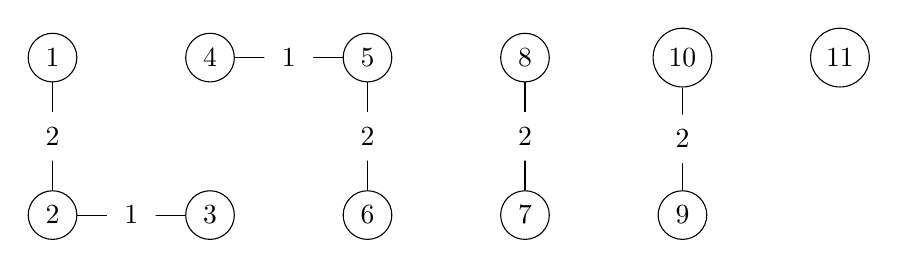
\begin{tikzpicture}

        \begin{scope}[every node/.style={circle,draw}]
          \node (1)  at (0,2)  {1};
          \node (2)  at (0,0)  {2};
          \node (3)  at (2,0)  {3};
          \node (4)  at (2,2)  {4};
          \node (5)  at (4,2)  {5};
          \node (6)  at (4,0)  {6};
          \node (7)  at (6,0)  {7};
          \node (8)  at (6,2)  {8};
          \node (9)  at (8,0)  {9};
          \node (10) at (8,2)  {10};
          \node (11) at (10,2) {11};
        \end{scope}

        \begin{scope}[every node/.style={fill=white,circle}]

          \begin{scope}[every edge/.style={draw}]
            \path (2)  edge node {$1$} (3);
            \path (4)  edge node {$1$} (5);
            \path (1)  edge node {$2$} (2);
            \path (5)  edge node {$2$} (6);
            \path (7)  edge node {$2$} (8);
            \path (9)  edge node {$2$} (10);
          \end{scope}
        \end{scope}

      \end{tikzpicture}
      \caption{[1, 5, 994, 219, 381]}
    \end{center}
  \end{figure}

  \begin{figure}[H]
    \begin{center}
      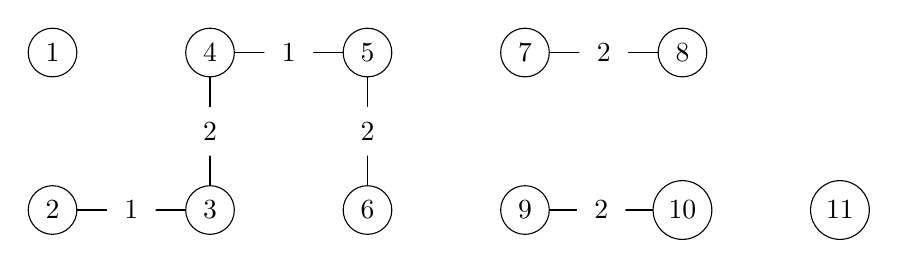
\begin{tikzpicture}

        \begin{scope}[every node/.style={circle,draw}]
          \node (1)  at (0,2)  {1};
          \node (2)  at (0,0)  {2};
          \node (3)  at (2,0)  {3};
          \node (4)  at (2,2)  {4};
          \node (5)  at (4,2)  {5};
          \node (6)  at (4,0)  {6};
          \node (7)  at (6,2)  {7};
          \node (8)  at (8,2)  {8};
          \node (9)  at (6,0)  {9};
          \node (10) at (8,0)  {10};
          \node (11) at (10,0) {11};
        \end{scope}

        \begin{scope}[every node/.style={fill=white,circle}]

          \begin{scope}[every edge/.style={draw}]
            \path (2)  edge node {$1$} (3);
            \path (4)  edge node {$1$} (5);
            \path (3)  edge node {$2$} (4);
            \path (5)  edge node {$2$} (6);
            \path (7)  edge node {$2$} (8);
            \path (9)  edge node {$2$} (10);
          \end{scope}
        \end{scope}

      \end{tikzpicture}
      \caption{[1, 5, 1010, 232, 381]}
    \end{center}
  \end{figure}

  \paragraph{}
  Dans le premier cas, $(\rho_1\rho_2)^2\rho_1$ nous donne ce que nous cherchons. Dans le second, c'est $(\rho_1\rho_2)^4\rho_1$ qui nous donne le résultat

\end{proof}

\paragraph{}
Grâce à ces deux théorèmes, on sait qu'il existe une 2-transposition $g$ dont $\rho_2$ est une extension qui est telle que $ g \in \Gamma_{0,1} = S_7$ et $g \in \Gamma_(0,3,4)$ donc $g \in \Gamma_{0,1} \cap \Gamma_(0,3,4)$ mais $g \notin \Gamma_{0,1,3,4} = <\rho_2>$. Donc $\Gamma_{0,1} \cap \Gamma_{0,3,4} \neq \Gamma_{0,1,3,4}$ donc $\Gamma$ ne satisafait pas la propriété d'intersection et n'est donc pas un C-group. Ce qui conclut la preuve du théorème
